In this chapter, the proof of concept for a simple serverless platform using WebAssembly technology will be explored. The platform utilizes an HTTP server to direct HTTP requests to specific WebAssembly modules. The popular Rust web framework, "Actix-web," has been chosen for the HTTP server implementation due to its lightweight and fast nature. Furthermore, the proof of concept employs Wasmtime as the Wasm-WASI runtime. As mentioned in the previous chapter, Wasmtime offers excellent support for the WASI standard and integrates various programming languages such as C++, Rust, Go, JavaScript, and more.

As Figure \ref{fig:poc} illustrates, this proof of concept assumes the availability of a function registry service that stores the ahead-of-time compiled Wasm binaries. Additionally, a serverless platform needs to be distributed; therefore, API gateways and load balancers are necessary to serve requests across the network. However, this proof of concept primarily focuses on the WebAssembly aspect of the platform, leaving the API gateway and load balancers outside the scope of the discussion.

\begin{figure}[H]
	\centering
		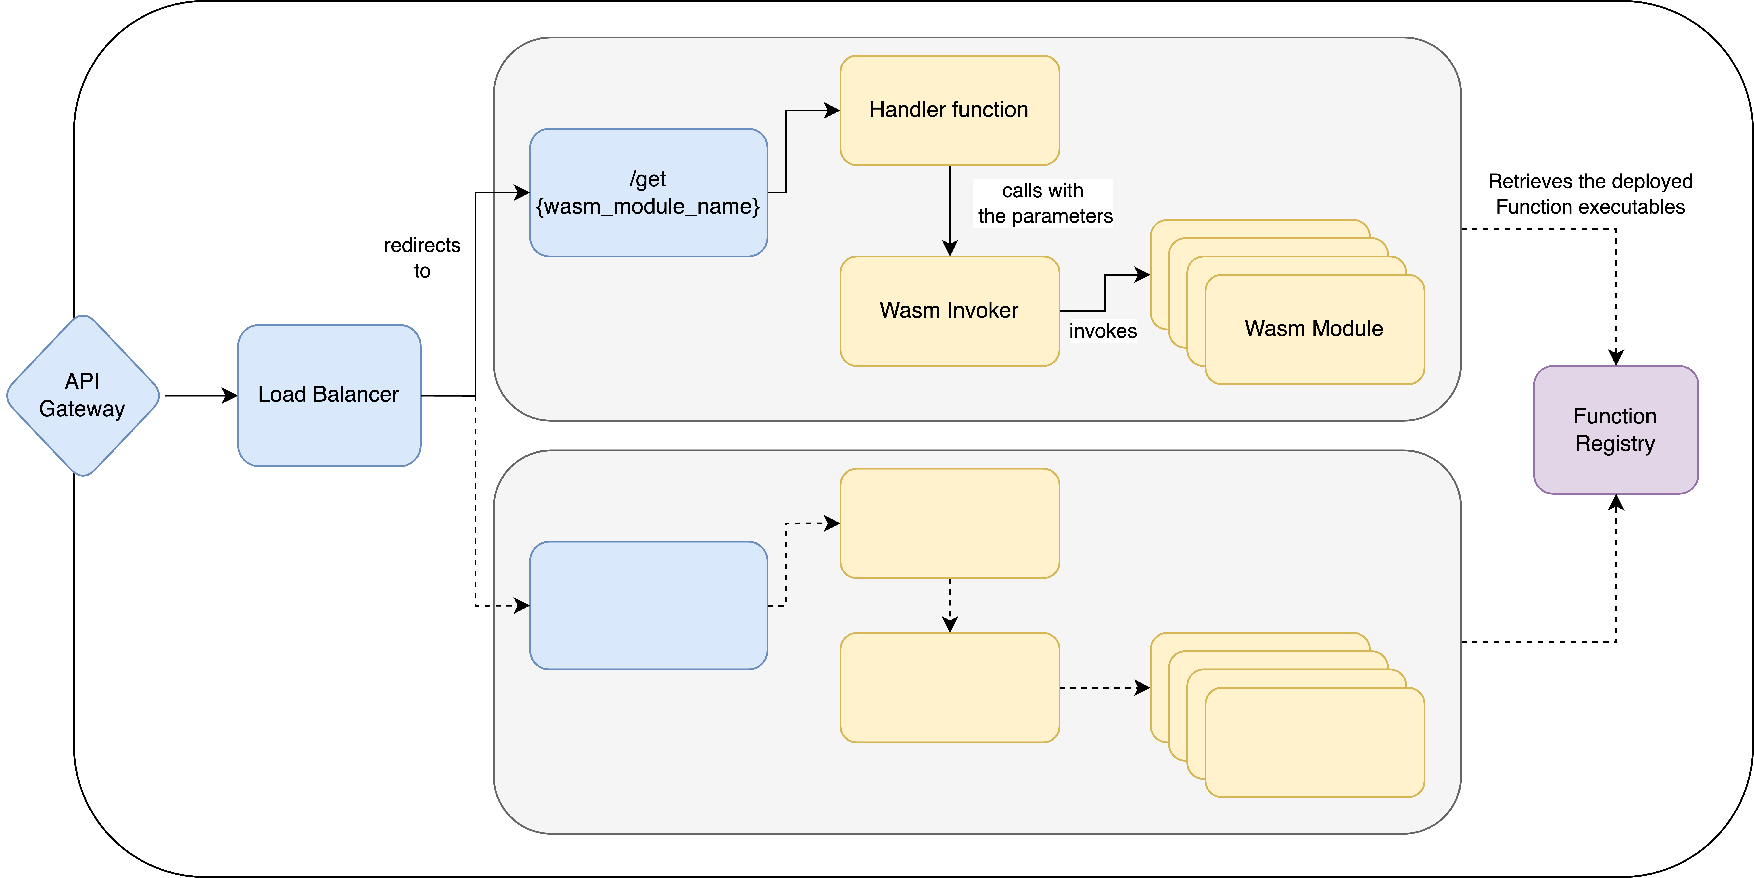
\includegraphics[width=1\linewidth]{images/poc/poc.pdf}
	\caption{Execution flow of the simple POC serverless platform}
	\label{fig:poc}
\end{figure}

%For this we need a WASI compliant Wasm modules, the fibonacci function from the previous chapter can be used here


\begin{lstlisting}[frame=lines, caption=actix http server with a handler function to invoce the wasm modules, captionpos=b, language=JavaScript, showstringspaces=false]
#[actix_web::main]
async fn main() -> io::Result<()> {
    HttpServer::new(|| App::new().service(handler))
        .bind("127.0.0.1:8080")?
        .run()
        .await
}

#[get("/{wasm_module_name}")]
async fn handler(
    wasm_module_name: Path<String>,
    query: Query<HashMap<String, String>>,
) -> impl Responder {
    let wasm_module = format!("{}.wasm", wasm_module_name);
    match invoke_wasm_module(wasm_module, query.into_inner()) {
        Ok(val) => HttpResponse::Ok().body(val),
        Err(e) => HttpResponse::InternalServerError().body(format!("Error: {}", e)),
    }
}

fn run_wasm_module(
    mut store: &mut Store<WasiCtx>,
    module: &Module,
    linker: &Linker<WasiCtx>,
) -> Result<()> {
    let instance = linker.instantiate(&mut store, module)?;
    let instance_main = instance.get_typed_func::<(), ()>(&mut store, "_start")?;
    Ok(instance_main.call(&mut store, ())?)
}
\end{lstlisting}


%Each stored Wasm module on the server is exposed by the handler function route, that takes the name of the Wasm module as a path parameter and loads the corresponding module.


